\begin{frame}{Regularization: Dropout}
    \framesubtitle{A Simple and Powerful Idea}
    \small
    \begin{itemize}
        \item \bhighlight{Dropout} is a regularization technique that prevents complex co-adaptations on training data by randomly dropping units (along with their connections) from the neural network during training.
        \item \textbf{The Core Idea:} In each forward pass, for each training example, we randomly set the output of some neurons to zero.
        \item The probability of keeping a neuron active is a hyperparameter, often set to 0.5.
    \end{itemize}
    \begin{figure}
        \centering
        % Source: Regularization.pdf, Page: 24
        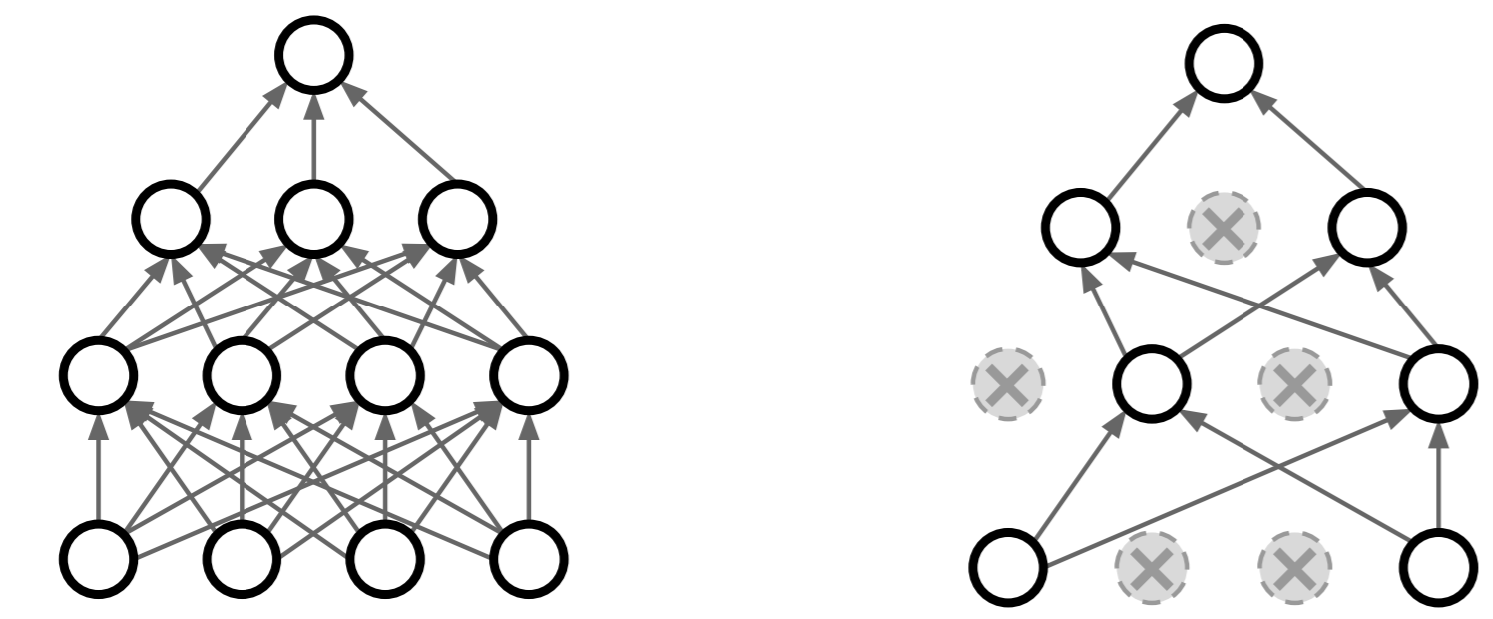
\includegraphics[width=0.7\linewidth]{images/dropout_idea.png}
        \caption{Left: A standard neural network. Right: The same network after applying dropout. Some neurons are temporarily deactivated.}
    \end{figure}
\end{frame}

\begin{frame}{Dropout: The Training Process}
    \framesubtitle{Training a Thinned Network}
    \small
    \begin{itemize}
        \item During each training step, we are effectively training a different, "thinned" version of the network for each mini-batch.
        \item The backpropagation step only updates the weights of the "active" neurons and connections for that specific forward pass.
        \item This forces the network to learn more robust and redundant features, as it cannot rely on any single neuron to be present.
    \end{itemize}
    \begin{figure}
        \centering
        % Source: Regularization.pdf, Page: 31
        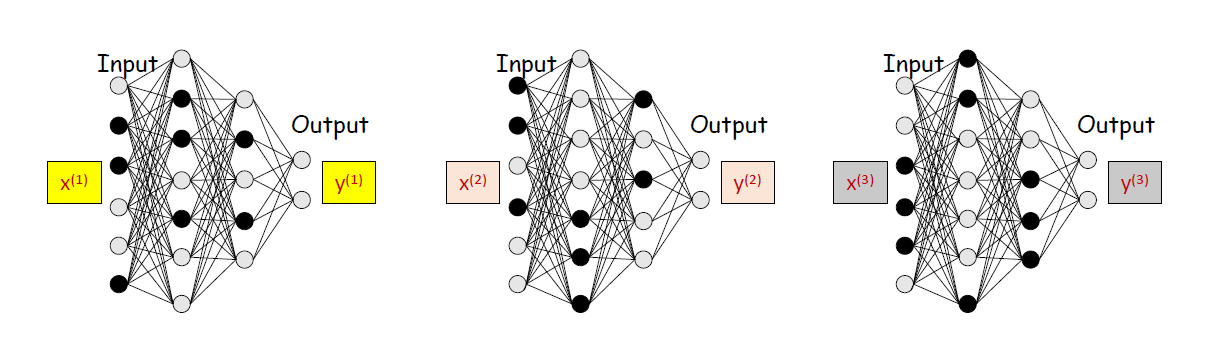
\includegraphics[width=\linewidth]{images/dropout_training_process.png}
        \caption{For each training example, a different random subset of neurons is deactivated, creating a unique "thinned" network.}
    \end{figure}
\end{frame}

\begin{frame}{Why Does Dropout Work?}
    \framesubtitle{Intuition 1: Preventing Co-adaptation}
    \small 
    \begin{itemize}
        \item Dropout prevents neurons from \bhighlight{co-adapting} too much.
        \item A neuron cannot rely on the presence of other specific neurons to correct its mistakes, because those other neurons might be dropped out at any time.
        \item Therefore, each neuron is forced to learn features that are useful on their own, leading to more robust and independent representations.
    \end{itemize}
    \begin{figure}
        \centering
        % Source: Regularization.pdf, Page: 29
        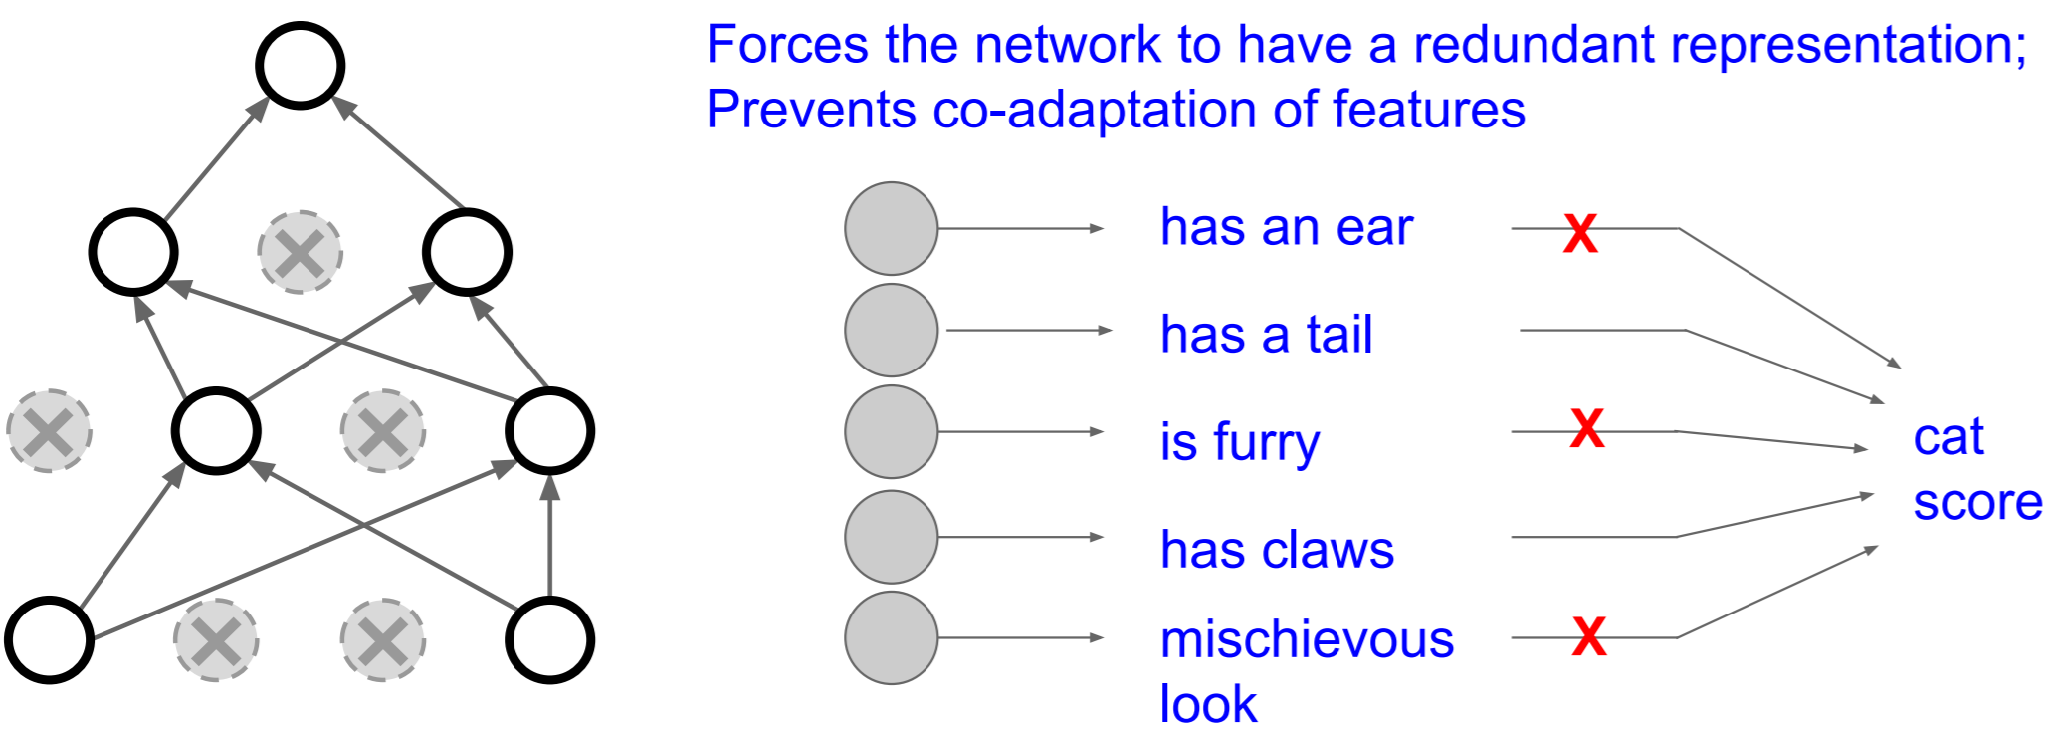
\includegraphics[width=0.8\linewidth]{images/dropout_coadaptation.png}
        \caption{Without dropout, a neuron might learn to rely on a specific feature (e.g., "has whiskers"). With dropout, it must learn from a more diverse set of features.}
    \end{figure}
\end{frame}

\begin{frame}{Why Does Dropout Work?}
    \framesubtitle{Intuition 2: An Ensemble of Networks}
    \small 
    \begin{itemize}
        \item Dropout can be viewed as an efficient way of training a huge \bhighlight{ensemble} of different neural networks.
        \item Each time we randomly drop out neurons, we are essentially training a different network architecture. For a network with N neurons, there are $2^N$ possible thinned networks!
        \item All these networks share weights, so we are effectively training an exponentially large number of models in parallel. At test time, we want to average their predictions.
    \end{itemize}
    \begin{figure}
        \centering
        % Source: Regularization.pdf, Page: 34
        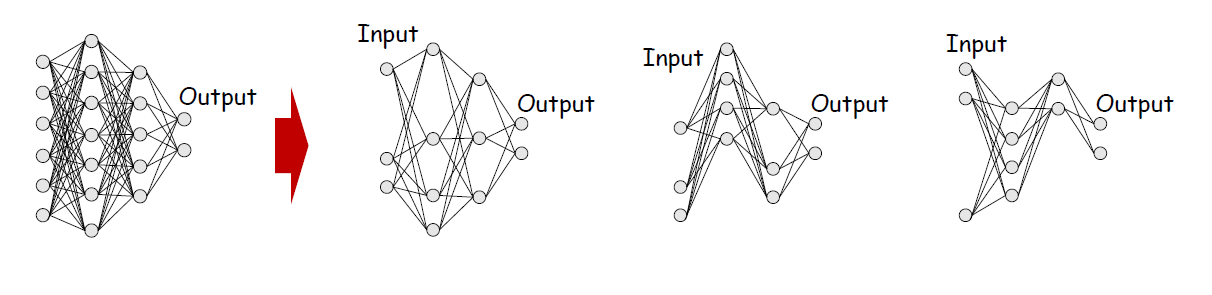
\includegraphics[width=\linewidth]{images/dropout_ensemble.png}
        \caption{Each dropout mask corresponds to training a different sub-network, but they all share the same underlying weights.}
    \end{figure}
\end{frame}

% --- SLIDE WITH CORRECTION ---
\begin{frame}{Dropout at Test Time}
    \framesubtitle{The Problem of Randomness}
    \begin{itemize}
        \item We cannot have random outputs at test time. We need a single, deterministic prediction.
        \item The ideal solution would be to average the predictions of all $2^N$ possible sub-networks, but this is computationally impossible.
        \item \textbf{A Simple Solution:} At test time, we use the full network with all neurons active, but we \bhighlight{scale down the weights} by the probability $p$ (the keep probability) that a neuron was active during training.
        \[ W_{\text{test}} = p \times W_{\text{train}} \]
    \end{itemize}
\end{frame}

\begin{frame}{Inverted Dropout}
    \framesubtitle{A More Common Implementation}
    \begin{itemize}
        \item A more common and practical method is \bhighlight{Inverted Dropout}.
        \item The key idea is to perform the scaling during \bhighlight{training time} instead of test time.
        \item During the forward pass of training, after dropping neurons, the activations of the remaining neurons are immediately scaled up by dividing by the keep probability $p$.
        \[ a^{[l]}_{\text{train}} = \frac{a^{[l]}_{\text{train}} * \text{mask}}{p} \]
        \item \textbf{Advantage:} The forward pass at test time remains completely unchanged. We don't need to do any extra scaling or modifications. This is much cleaner to implement.
    \end{itemize}
\end{frame}

\begin{frame}{Dropout: Practical Considerations}
    \framesubtitle{Tips and Trade-offs}
    \begin{itemize}
        \item \textbf{When to use it:} If your network is significantly overfitting, Dropout is a very effective regularizer.
        \item \textbf{Training Time:} Training with dropout typically takes longer to converge because the gradient updates are noisier and each neuron is trained less often.
        \item \textbf{Dropout Strength:} The keep probability $p$ (often between 0.5 and 0.8) is a hyperparameter you need to tune. A lower $p$ means stronger regularization.
        \item \textbf{Interaction with Batch Norm:} Some evidence suggests that Batch Normalization can reduce the need for Dropout. Using both might not always provide additional benefits.
    \end{itemize}
\end{frame}

\begin{frame}{Dropout: Typical Results}
    \framesubtitle{Impact on Generalization}
    \begin{figure}
        \centering
        % Source: Regularization.pdf, Page: 47
        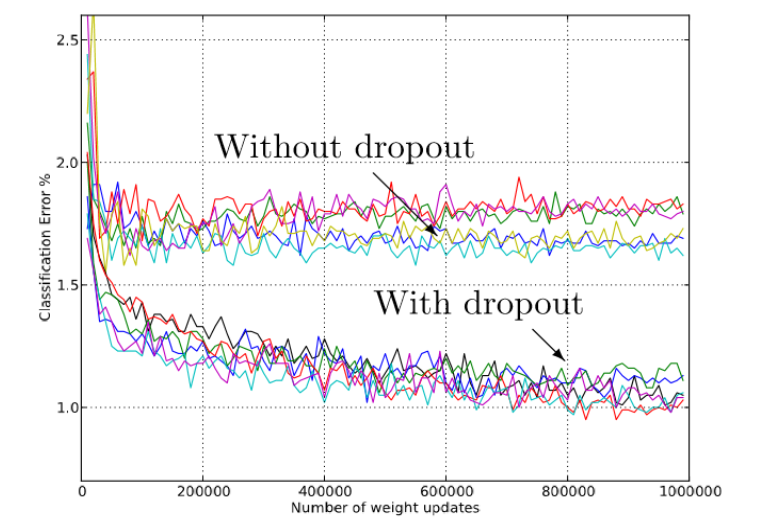
\includegraphics[width=0.9\linewidth]{images/dropout_results.png}
        \caption{A typical result showing that a network trained \textbf{with dropout} (bottom curves) achieves a lower classification error on the test set compared to the same network trained \textbf{without dropout} (top curves).}
    \end{figure}
\end{frame}